\documentclass{standalone}
\usepackage{tikz}
\usetikzlibrary{patterns, positioning}
\usepackage[sfdefault]{ClearSans} %% option 'sfdefault' activates Clear Sans as the default text font
\usepackage[T1]{fontenc}

\begin{document}
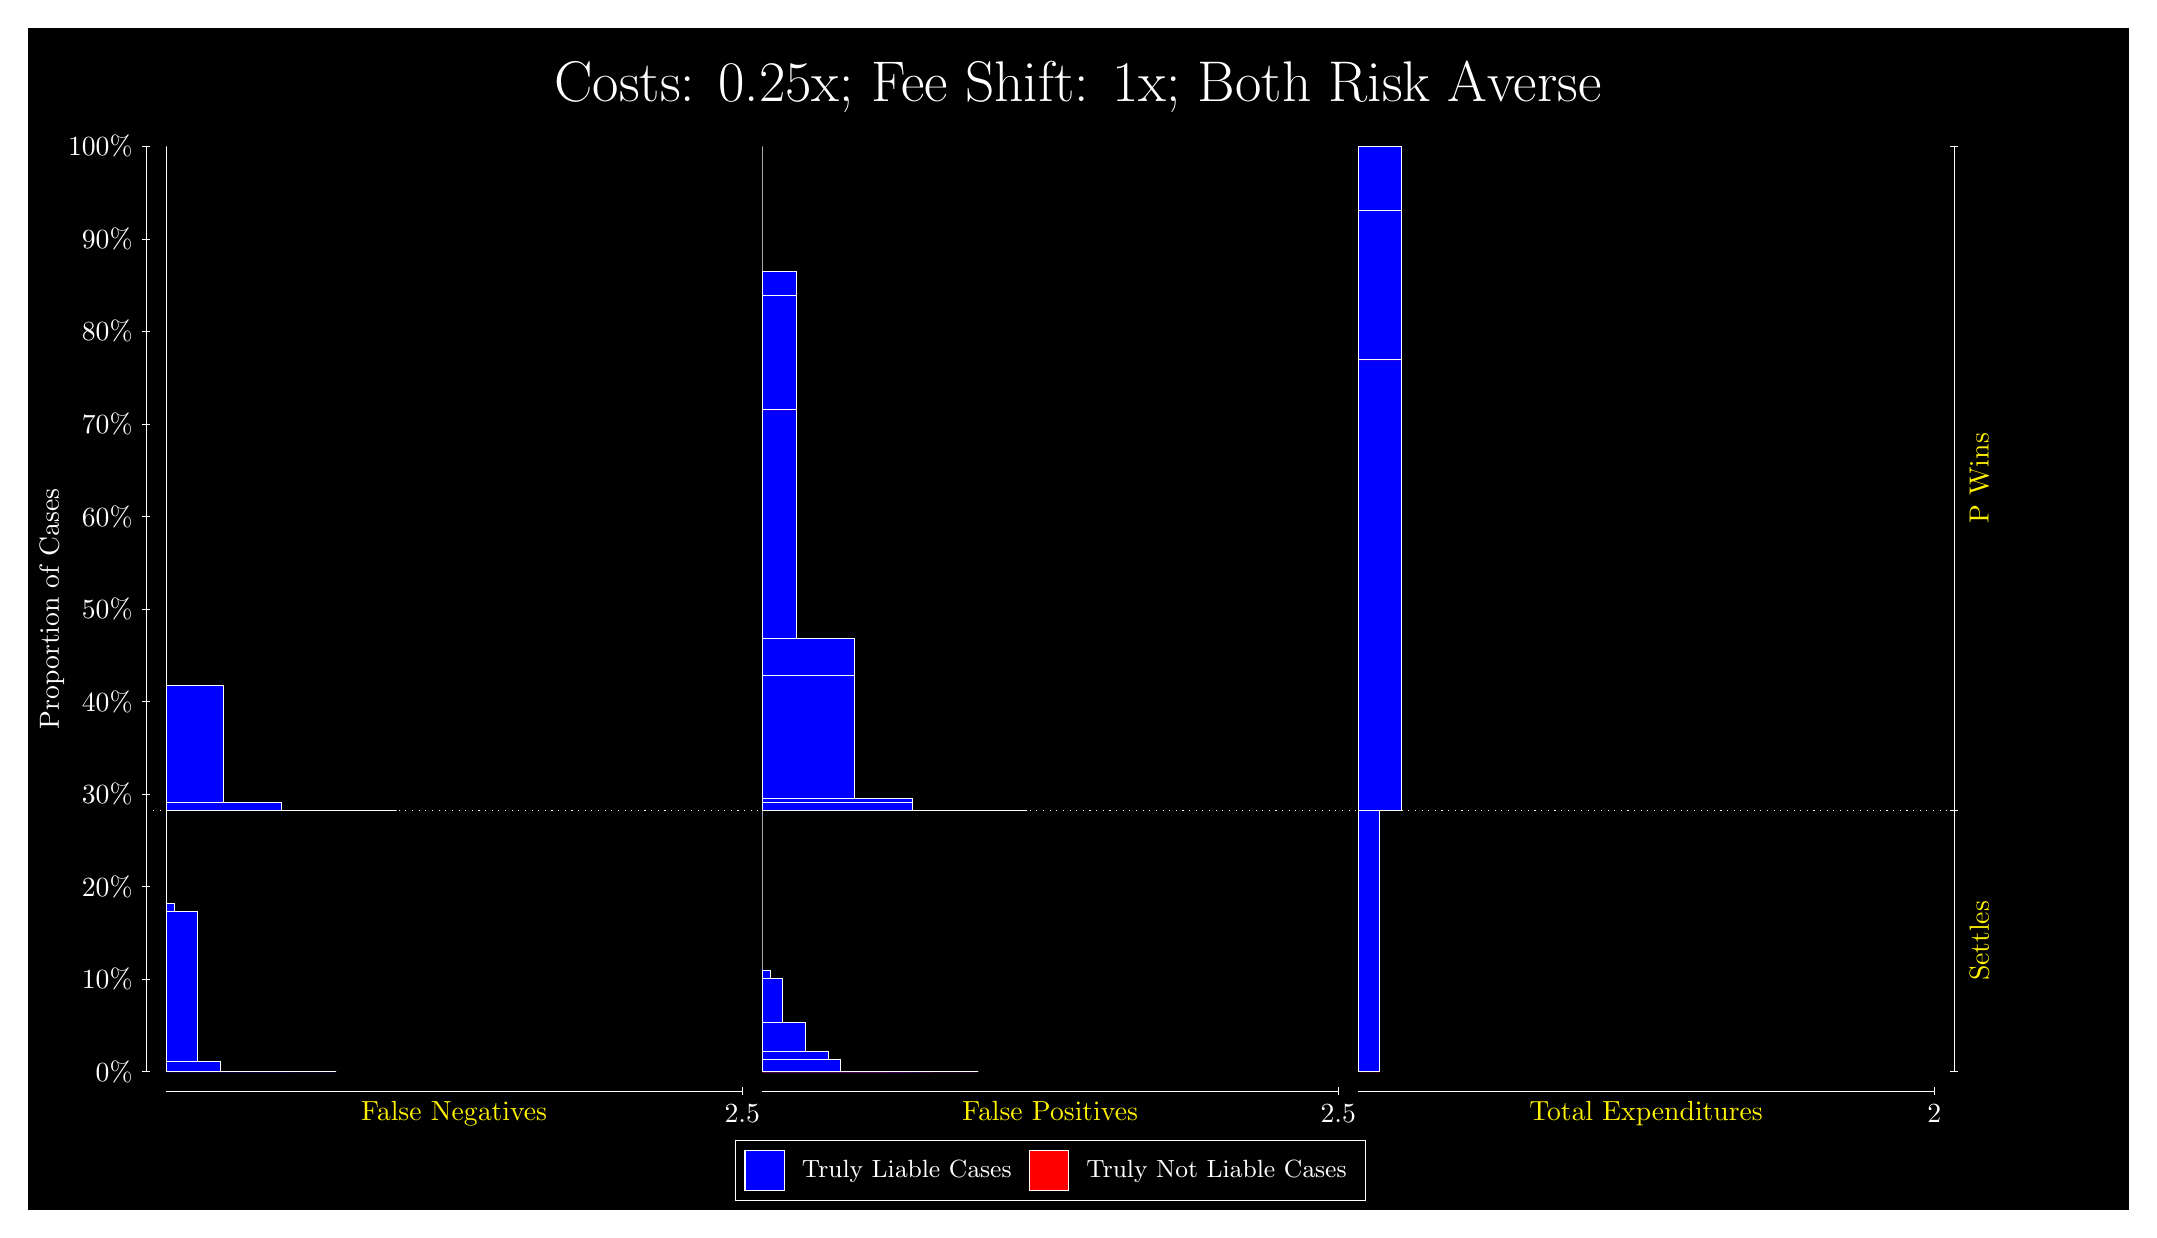
\begin{tikzpicture}
\draw[fill=black] (0,0) rectangle (26.667,15);
\draw[text=white] (0,13.5) rectangle (26.667,15) node[midway] {\huge Costs: 0.25x; Fee Shift: 1x; Both Risk Averse};
\draw[white, very thin] (1.5,1.75) -- (1.5,13.5);
\node[rotate=90, text=white, anchor=center] at (0.3, 7.625) {Proportion of Cases};
\draw[white, very thin] (1.45,1.75) -- (1.55,1.75);
\node[text=white, anchor=east] at (1.45, 1.75) {0\%};
\draw[white, very thin] (1.45,2.925) -- (1.55,2.925);
\node[text=white, anchor=east] at (1.45, 2.925) {10\%};
\draw[white, very thin] (1.45,4.1) -- (1.55,4.1);
\node[text=white, anchor=east] at (1.45, 4.1) {20\%};
\draw[white, very thin] (1.45,5.275) -- (1.55,5.275);
\node[text=white, anchor=east] at (1.45, 5.275) {30\%};
\draw[white, very thin] (1.45,6.45) -- (1.55,6.45);
\node[text=white, anchor=east] at (1.45, 6.45) {40\%};
\draw[white, very thin] (1.45,7.625) -- (1.55,7.625);
\node[text=white, anchor=east] at (1.45, 7.625) {50\%};
\draw[white, very thin] (1.45,8.8) -- (1.55,8.8);
\node[text=white, anchor=east] at (1.45, 8.8) {60\%};
\draw[white, very thin] (1.45,9.975) -- (1.55,9.975);
\node[text=white, anchor=east] at (1.45, 9.975) {70\%};
\draw[white, very thin] (1.45,11.15) -- (1.55,11.15);
\node[text=white, anchor=east] at (1.45, 11.15) {80\%};
\draw[white, very thin] (1.45,12.325) -- (1.55,12.325);
\node[text=white, anchor=east] at (1.45, 12.325) {90\%};
\draw[white, very thin] (1.45,13.5) -- (1.55,13.5);
\node[text=white, anchor=east] at (1.45, 13.5) {100\%};

\draw[white, very thin] (24.457,1.75) -- (24.457,13.5);
\draw[white, very thin] (24.407,1.75) -- (24.507,1.75);
\node[anchor=west] at (24.407, 1.75) {};
\draw[white, very thin] (24.407,5.0688) -- (24.507,5.0688);
\node[anchor=west] at (24.407, 5.0688) {};
\draw[white, very thin] (24.407,13.5) -- (24.507,13.5);
\node[anchor=west] at (24.407, 13.5) {};

\draw[white, very thin, fill=blue] (1.75,1.75) rectangle (3.9091,1.75);
\draw[white, very thin, fill=blue] (1.75,1.75) rectangle (3.3236,1.75);
\draw[white, very thin, fill=blue] (1.75,1.75) rectangle (3.1772,1.7509);
\draw[white, very thin, fill=blue] (1.75,1.7509) rectangle (3.0308,1.7509);
\draw[white, very thin, fill=blue] (1.75,1.7509) rectangle (2.738,1.7509);
\draw[white, very thin, fill=blue] (1.75,1.7509) rectangle (2.5917,1.7518);
\draw[white, very thin, fill=blue] (1.75,1.7518) rectangle (2.4453,1.8757);
\draw[white, very thin, fill=blue] (1.75,1.8757) rectangle (2.2989,1.8759);
\draw[white, very thin, fill=blue] (1.75,1.8759) rectangle (2.1525,3.7827);
\draw[white, very thin, fill=blue] (1.75,3.7827) rectangle (2.0062,3.7829);
\draw[white, very thin, fill=blue] (1.75,3.7829) rectangle (1.8598,3.8873);
\draw[white, very thin, fill=red] (1.75,3.8873) rectangle (1.75,3.8873);
\draw[white, very thin, fill=blue] (1.75,3.8873) rectangle (1.75,5.0688);
\draw[white, very thin, fill=blue] (1.75,5.0688) rectangle (4.6775,5.0688);
\draw[white, very thin, fill=blue] (1.75,5.0688) rectangle (3.9457,5.0699);
\draw[white, very thin, fill=blue] (1.75,5.0699) rectangle (3.2138,5.1757);
\draw[white, very thin, fill=blue] (1.75,5.1757) rectangle (2.4819,6.6614);
\draw[white, very thin, fill=red] (1.75,6.6614) rectangle (1.75,6.6614);
\draw[white, very thin, fill=blue] (1.75,6.6614) rectangle (1.75,13.5);
\draw[white, very thin, fill=red] (9.3189,1.75) rectangle (12.063,1.75);
\draw[white, very thin, fill=blue] (9.3189,1.75) rectangle (12.063,1.75);
\draw[white, very thin, fill=red] (9.3189,1.75) rectangle (11.478,1.75);
\draw[white, very thin, fill=blue] (9.3189,1.75) rectangle (11.478,1.75);
\draw[white, very thin, fill=blue] (9.3189,1.75) rectangle (11.332,1.75);
\draw[white, very thin, fill=red] (9.3189,1.75) rectangle (11.185,1.75);
\draw[white, very thin, fill=blue] (9.3189,1.75) rectangle (11.185,1.75);
\draw[white, very thin, fill=red] (9.3189,1.75) rectangle (10.892,1.75);
\draw[white, very thin, fill=blue] (9.3189,1.75) rectangle (10.892,1.7513);
\draw[white, very thin, fill=blue] (9.3189,1.7513) rectangle (10.746,1.7513);
\draw[white, very thin, fill=blue] (9.3189,1.7513) rectangle (10.6,1.7541);
\draw[white, very thin, fill=blue] (9.3189,1.7541) rectangle (10.453,1.7541);
\draw[white, very thin, fill=red] (9.3189,1.7541) rectangle (10.307,1.7541);
\draw[white, very thin, fill=blue] (9.3189,1.7541) rectangle (10.307,1.9016);
\draw[white, very thin, fill=blue] (9.3189,1.9016) rectangle (10.161,2.0063);
\draw[white, very thin, fill=blue] (9.3189,2.0063) rectangle (10.014,2.0064);
\draw[white, very thin, fill=blue] (9.3189,2.0064) rectangle (9.8678,2.3763);
\draw[white, very thin, fill=blue] (9.3189,2.3763) rectangle (9.7214,2.3765);
\draw[white, very thin, fill=blue] (9.3189,2.3765) rectangle (9.575,2.9316);
\draw[white, very thin, fill=blue] (9.3189,2.9316) rectangle (9.4287,3.036);
\draw[white, very thin, fill=blue] (9.3189,3.036) rectangle (9.3189,5.0688);
\draw[white, very thin, fill=red] (9.3189,5.0688) rectangle (12.686,5.0688);
\draw[white, very thin, fill=blue] (9.3189,5.0688) rectangle (12.686,5.0688);
\draw[white, very thin, fill=red] (9.3189,5.0688) rectangle (11.954,5.0688);
\draw[white, very thin, fill=blue] (9.3189,5.0688) rectangle (11.954,5.0701);
\draw[white, very thin, fill=blue] (9.3189,5.0701) rectangle (11.954,5.0708);
\draw[white, very thin, fill=red] (9.3189,5.0708) rectangle (11.222,5.0708);
\draw[white, very thin, fill=blue] (9.3189,5.0708) rectangle (11.222,5.1752);
\draw[white, very thin, fill=blue] (9.3189,5.1752) rectangle (11.222,5.2225);
\draw[white, very thin, fill=red] (9.3189,5.2225) rectangle (10.49,5.2225);
\draw[white, very thin, fill=blue] (9.3189,5.2225) rectangle (10.49,6.7835);
\draw[white, very thin, fill=blue] (9.3189,6.7835) rectangle (10.49,7.2485);
\draw[white, very thin, fill=blue] (9.3189,7.2485) rectangle (9.758,10.156);
\draw[white, very thin, fill=red] (9.3189,10.156) rectangle (9.758,10.156);
\draw[white, very thin, fill=blue] (9.3189,10.156) rectangle (9.758,11.614);
\draw[white, very thin, fill=blue] (9.3189,11.614) rectangle (9.758,11.907);
\draw[white, very thin, fill=blue] (9.3189,11.907) rectangle (9.3189,13.5);
\draw[white, very thin, fill=red] (16.888,1.75) rectangle (17.162,1.75);
\draw[white, very thin, fill=blue] (16.888,1.75) rectangle (17.162,5.0688);
\draw[white, very thin, fill=red] (16.888,5.0688) rectangle (17.437,5.0688);
\draw[white, very thin, fill=blue] (16.888,5.0688) rectangle (17.437,10.79);
\draw[white, very thin, fill=red] (16.888,10.79) rectangle (17.437,10.79);
\draw[white, very thin, fill=blue] (16.888,10.79) rectangle (17.437,12.693);
\draw[white, very thin, fill=red] (16.888,12.693) rectangle (17.437,12.693);
\draw[white, very thin, fill=blue] (16.888,12.693) rectangle (17.437,13.5);
\draw[white, dotted] (1.5,5.0688) -- (24.457,5.0688);
\draw[white, very thin] (1.75,1.5) -- (9.0689,1.5);
\node[text=yellow, anchor=north] at (5.4094, 1.5) {False Negatives};
\draw[white, very thin] (9.0689,1.45) -- (9.0689,1.55);
\node[text=white, anchor=north] at (9.0689, 1.45) {2.5};

\draw[white, very thin] (9.3189,1.5) -- (16.638,1.5);
\node[text=yellow, anchor=north] at (12.978, 1.5) {False Positives};
\draw[white, very thin] (16.638,1.45) -- (16.638,1.55);
\node[text=white, anchor=north] at (16.638, 1.45) {2.5};

\draw[white, very thin] (16.888,1.5) -- (24.207,1.5);
\node[text=yellow, anchor=north] at (20.547, 1.5) {Total Expenditures};
\draw[white, very thin] (24.207,1.45) -- (24.207,1.55);
\node[text=white, anchor=north] at (24.207, 1.45) {2};

\node[text=yellow, centered, rotate=90] at (24.777, 3.4094) {Settles};
\node[text=yellow, centered, rotate=90] at (24.777, 9.2844) {P Wins};

\draw (12.978300999999998,1.5) node[draw=none] (baseCoordinate) {};
\begin{scope}[align=center]
        \matrix[scale=0.5, draw=white, below=0.5cm of baseCoordinate, nodes={draw}, column sep=0.1cm]{
            \node[rectangle, draw, minimum width=0.5cm, minimum height=0.5cm, fill=blue] {}; &
            \node[draw=none, font=\small, text=white] (B) {Truly Liable Cases}; &
            \node[rectangle, draw, minimum width=0.5cm, minimum height=0.5cm, fill=red] {}; &
            \node[draw=none, font=\small, text=white] (B) {Truly Not Liable Cases}; \\
            };
\end{scope}

\end{tikzpicture}
\end{document}